% ============================================================
\chapter{Linear Systems and Phase Portrait Classification}
\label{ch:linear}
% ============================================================

\section{Introduction}

Before confronting the whirlwinds of chaos and the complexity of nonlinear systems, one must master the linear case---the one where everything can be computed explicitly. The phase portrait of a planar linear system is entirely determined by the eigenvalues of its matrix: stable or unstable nodes, spiralling foci, elliptic centres, saddle points. This classification, inherited from the work of Poincar\'e and his student Ivar Bendixson at the end of the nineteenth century, constitutes the visual dictionary that every dynamicist consults first.

But the linear system is more than a pedagogical exercise. Thanks to the Hartman-Grobman theorem, the linearised phase portrait near a hyperbolic equilibrium faithfully reproduces the local behaviour of the nonlinear system. This is why linear systems constitute the fundamental building block of dynamical systems
theory. This chapter develops the
complete classification of phase portraits for planar systems
$\dot{x} = Ax$, $x \in \R^2$.

\section{General Solution and Matrix Exponential}

\begin{theorem}[Solution of the linear system]
The solution of $\dot{x} = Ax$ with initial condition $x(0) = x_0$ is
\[
    x(t) = e^{At}\, x_0,
\]
where the \textbf{matrix exponential} is defined by
\[
    e^{At} = \sum_{k=0}^{+\infty} \frac{(At)^k}{k!} = I + At + \frac{A^2 t^2}{2!} + \cdots
\]
\end{theorem}

\begin{proposition}[Properties of $e^{At}$]
\begin{enumerate}
    \item $e^{A \cdot 0} = I$;
    \item $\frac{d}{dt} e^{At} = A e^{At} = e^{At} A$;
    \item $e^{A(t+s)} = e^{At}\, e^{As}$;
    \item $(e^{At})^{-1} = e^{-At}$;
    \item If $P$ is invertible, $e^{(P^{-1}AP)t} = P^{-1} e^{At} P$;
    \item $\det(e^{At}) = e^{\mathrm{tr}(A)\, t}$.
\end{enumerate}
\end{proposition}

\begin{keyformulas}[title=\textbf{Computing $e^{At}$ for $A \in \R^{2 \times 2}$}]
If $A$ has eigenvalues $\lambda_1, \lambda_2$:
\begin{itemize}
    \item \textbf{Distinct real eigenvalues}:
    $e^{At} = \frac{\lambda_2 e^{\lambda_1 t} - \lambda_1 e^{\lambda_2 t}}{\lambda_2 - \lambda_1} I
    + \frac{e^{\lambda_2 t} - e^{\lambda_1 t}}{\lambda_2 - \lambda_1} A$.
    \item \textbf{Repeated eigenvalue $\lambda$}:
    $e^{At} = e^{\lambda t}(I + (A - \lambda I)t)$ if $A \neq \lambda I$.
    \item \textbf{Complex eigenvalues $\lambda = \alpha \pm i\beta$}:
    $e^{At} = e^{\alpha t}\left(\cos(\beta t)\, I + \frac{\sin(\beta t)}{\beta}(A - \alpha I)\right)$.
\end{itemize}
\end{keyformulas}

\section{Classification in $\R^2$}

Consider the system $\dot{x} = Ax$ where $A \in \R^{2\times 2}$ and
$\det(A) \neq 0$ (the origin is the unique equilibrium). The relevant
invariants are:
\begin{itemize}
    \item $\tau = \mathrm{tr}(A) = \lambda_1 + \lambda_2$;
    \item $\delta = \det(A) = \lambda_1 \lambda_2$;
    \item $\Delta = \tau^2 - 4\delta$ (discriminant of the characteristic polynomial).
\end{itemize}

\subsection{Stable Node ($\lambda_1 < \lambda_2 < 0$)}

\begin{definition}[Stable node]
The phase portrait is a \textbf{stable node} when both eigenvalues are real
and strictly negative. All orbits converge to the origin, tangent to the
eigenspace of the eigenvalue with largest modulus.
\end{definition}

Conditions: $\delta > 0$, $\tau < 0$, $\Delta > 0$.

\begin{center}
\begin{tikzpicture}
    \begin{axis}[
        width=7cm, height=7cm,
        xlabel={$x_1$}, ylabel={$x_2$},
        xmin=-3, xmax=3, ymin=-3, ymax=3,
        axis lines=middle, ticks=none,
        title={Stable node}
    ]
    \addplot[blue, thick, ->, domain=0:2.5, samples=50] ({2.5*exp(-x)*cos(30)}, {2.5*exp(-2*x)*sin(30)});
    \addplot[blue, thick, ->, domain=0:2.5, samples=50] ({-2*exp(-x)*cos(20)}, {2*exp(-2*x)*sin(50)});
    \addplot[blue, thick, ->, domain=0:2.5, samples=50] ({1.5*exp(-x)}, {-2*exp(-2*x)});
    \addplot[blue, thick, ->, domain=0:2.5, samples=50] ({-2*exp(-x)}, {-1.5*exp(-2*x)});
    \node at (axis cs:0,0) [circle, fill=black, inner sep=1.5pt] {};
    \end{axis}
\end{tikzpicture}
\end{center}

\subsection{Unstable Node ($0 < \lambda_1 < \lambda_2$)}

\begin{definition}[Unstable node]
The phase portrait is symmetric to the stable node: orbits diverge from the
origin. Conditions: $\delta > 0$, $\tau > 0$, $\Delta > 0$.
\end{definition}

\subsection{Saddle Point ($\lambda_1 < 0 < \lambda_2$)}

\begin{definition}[Saddle point]
The phase portrait is a \textbf{saddle point} when the eigenvalues have
opposite signs. Orbits approach the origin along the stable eigenspace and
recede along the unstable eigenspace.
\end{definition}

Conditions: $\delta < 0$.

\begin{center}
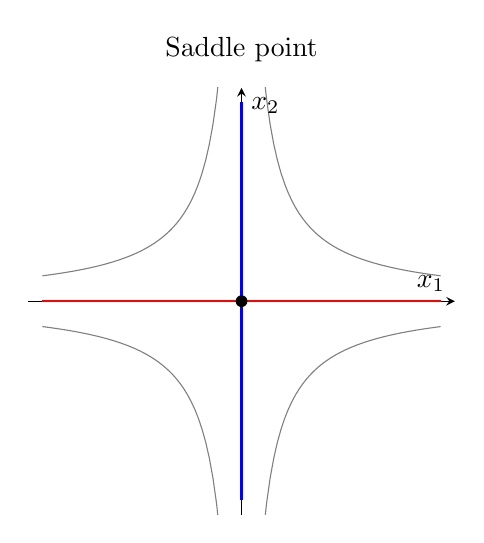
\begin{tikzpicture}
    \begin{axis}[
        width=7cm, height=7cm,
        xlabel={$x_1$}, ylabel={$x_2$},
        xmin=-3, xmax=3, ymin=-3, ymax=3,
        axis lines=middle, ticks=none,
        title={Saddle point}
    ]
    \addplot[red, thick, domain=-2.8:2.8, samples=2] {0};
    \addplot[blue, thick, domain=-2.8:2.8, samples=50] ({0}, {x});
    \addplot[gray, domain=0.3:2.8, samples=50] {1/x};
    \addplot[gray, domain=0.3:2.8, samples=50] {-1/x};
    \addplot[gray, domain=-2.8:-0.3, samples=50] {1/x};
    \addplot[gray, domain=-2.8:-0.3, samples=50] {-1/x};
    \node at (axis cs:0,0) [circle, fill=black, inner sep=1.5pt] {};
    \end{axis}
\end{tikzpicture}
\end{center}

\subsection{Stable Focus ($\lambda = \alpha \pm i\beta$, $\alpha < 0$)}

\begin{definition}[Stable focus]
The phase portrait is a \textbf{stable focus} (or stable spiral) when the
eigenvalues are complex conjugates with negative real part. Orbits spiral
toward the origin.
\end{definition}

Conditions: $\Delta < 0$, $\tau < 0$.

\subsection{Unstable Focus ($\alpha > 0$)}

Symmetric portrait: diverging spirals. Conditions: $\Delta < 0$, $\tau > 0$.

\subsection{Center ($\lambda = \pm i\beta$, $\alpha = 0$)}

\begin{definition}[Center]
The phase portrait is a \textbf{center} when the eigenvalues are purely
imaginary. Orbits are closed ellipses around the origin. The equilibrium is
stable but not asymptotically stable.
\end{definition}

Conditions: $\Delta < 0$, $\tau = 0$.

\begin{warning}[title=\textbf{Centers and nonlinear perturbations}]
A linear center is \emph{structurally unstable}: an arbitrarily small
nonlinear perturbation can turn it into a focus (stable or unstable). This is
a critical case for linearization.
\end{warning}

\subsection{Degenerate Node and Star Node}

\begin{definition}[Star node]
If $A = \lambda I$ ($\lambda < 0$), every line through the origin is an orbit:
this is a \textbf{stable star node}.
\end{definition}

\begin{definition}[Degenerate node]
If $A$ has a double eigenvalue $\lambda < 0$ with only one eigenvector
(Jordan block), the phase portrait is a \textbf{stable degenerate node}.
All orbits are tangent to the eigenspace.
\end{definition}

\section{The $(\tau, \delta)$ Diagram}

The complete classification is summarized in the $(\tau, \delta)$ plane:

\begin{center}
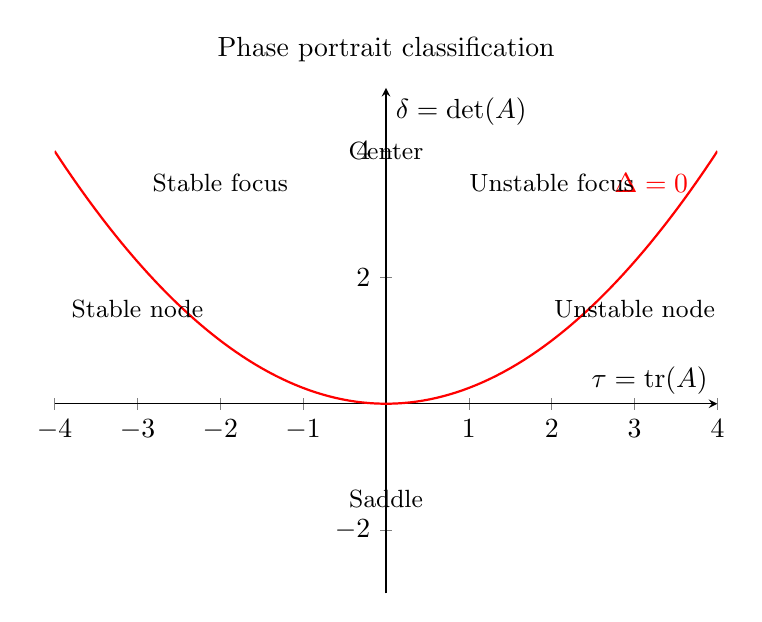
\begin{tikzpicture}
    \begin{axis}[
        width=10cm, height=8cm,
        xlabel={$\tau = \mathrm{tr}(A)$},
        ylabel={$\delta = \det(A)$},
        xmin=-4, xmax=4, ymin=-3, ymax=5,
        axis lines=middle,
        title={Phase portrait classification}
    ]
    \addplot[thick, red, domain=-4:4, samples=100] {x^2/4};
    \node[red] at (axis cs:3.2,3.5) {$\Delta=0$};
    \node at (axis cs:-2,3.5) {\small Stable focus};
    \node at (axis cs:2,3.5) {\small Unstable focus};
    \node at (axis cs:0,4) {\small Center};
    \node at (axis cs:-3,1.5) {\small Stable node};
    \node at (axis cs:3,1.5) {\small Unstable node};
    \node at (axis cs:0,-1.5) {\small Saddle};
    \end{axis}
\end{tikzpicture}
\end{center}

\begin{theorem}[Complete classification in dimension 2]
Let $A \in \R^{2\times 2}$ with $\det(A) \neq 0$. The nature of the phase
portrait of $\dot{x} = Ax$ is entirely determined by
$\tau = \mathrm{tr}(A)$ and $\delta = \det(A)$:
\begin{center}
\begin{tabular}{lll}
\hline
\textbf{Type} & \textbf{Conditions} & \textbf{Stability} \\
\hline
Stable node & $\delta > 0$, $\tau < 0$, $\Delta \geq 0$ & Asymp.\ stable \\
Unstable node & $\delta > 0$, $\tau > 0$, $\Delta \geq 0$ & Unstable \\
Saddle & $\delta < 0$ & Unstable \\
Stable focus & $\Delta < 0$, $\tau < 0$ & Asymp.\ stable \\
Unstable focus & $\Delta < 0$, $\tau > 0$ & Unstable \\
Center & $\Delta < 0$, $\tau = 0$ & Stable (not asymp.) \\
\hline
\end{tabular}
\end{center}
\end{theorem}

\section{Linear Systems in Higher Dimensions}

\subsection{Decomposition into Invariant Subspaces}

\begin{theorem}[Spectral decomposition]
Let $A \in \R^{n \times n}$. The space $\R^n$ decomposes as a direct sum
of invariant subspaces:
\[
    \R^n = E^s \oplus E^u \oplus E^c,
\]
where:
\begin{itemize}
    \item $E^s$ (\textbf{stable} subspace): generalized eigenvalues with
    real part $< 0$;
    \item $E^u$ (\textbf{unstable} subspace): generalized eigenvalues with
    real part $> 0$;
    \item $E^c$ (\textbf{center} subspace): generalized eigenvalues with
    real part $= 0$.
\end{itemize}
\end{theorem}

\begin{proposition}[Asymptotic behavior]
\begin{enumerate}
    \item For $x_0 \in E^s$: $\norm{e^{At} x_0} \to 0$ exponentially as
    $t \to +\infty$.
    \item For $x_0 \in E^u$: $\norm{e^{At} x_0} \to +\infty$ exponentially
    as $t \to +\infty$.
    \item For $x_0 \in E^c$: $\norm{e^{At} x_0}$ grows at most polynomially.
\end{enumerate}
\end{proposition}

\subsection{Jordan Form and Exponential}

\begin{proposition}[Exponential of a Jordan block]
If $J_k(\lambda) = \lambda I_k + N_k$ is a Jordan block of size $k$, then
\[
    e^{J_k(\lambda)t} = e^{\lambda t}
    \begin{pmatrix}
        1 & t & \frac{t^2}{2} & \cdots & \frac{t^{k-1}}{(k-1)!} \\
        0 & 1 & t & \cdots & \frac{t^{k-2}}{(k-2)!} \\
        \vdots & & \ddots & & \vdots \\
        0 & 0 & \cdots & 1 & t \\
        0 & 0 & \cdots & 0 & 1
    \end{pmatrix}.
\]
\end{proposition}

\section{Non-autonomous Linear Systems}

\begin{definition}[Fundamental matrix]
For the system $\dot{x} = A(t)\, x$, a \textbf{fundamental matrix} is a
matrix $\Phi(t) \in \R^{n \times n}$ whose columns form a fundamental set
of solutions. It satisfies $\dot{\Phi}(t) = A(t)\, \Phi(t)$ and
$\det(\Phi(t)) \neq 0$.
\end{definition}

\begin{theorem}[Liouville-Jacobi formula]
$\det(\Phi(t)) = \det(\Phi(t_0))\, \exp\!\left(\int_{t_0}^t \mathrm{tr}(A(s))\, ds\right)$.
\end{theorem}

\section{Applications}

\begin{example}[RLC circuit]
A series RLC circuit is governed by
\[
    L\ddot{q} + R\dot{q} + \frac{q}{C} = 0,
\]
yielding with $x_1 = q$, $x_2 = \dot{q}$:
\[
    A = \begin{pmatrix} 0 & 1 \\ -\frac{1}{LC} & -\frac{R}{L} \end{pmatrix}.
\]
Depending on the values of $R$, $L$, $C$:
\begin{itemize}
    \item $R^2 < 4L/C$: stable focus (damped oscillations);
    \item $R^2 = 4L/C$: degenerate node (critical damping);
    \item $R^2 > 4L/C$: stable node (overdamping).
\end{itemize}
\end{example}

\begin{codeblock}[title=\textbf{Phase portraits for different matrices}]
\begin{minted}{python}
import numpy as np
import matplotlib.pyplot as plt
from scipy.integrate import solve_ivp

matrices = {
    "Stable node": np.array([[-2, 0], [0, -1]]),
    "Saddle": np.array([[-1, 0], [0, 1]]),
    "Stable focus": np.array([[-0.5, 2], [-2, -0.5]]),
    "Center": np.array([[0, 1], [-1, 0]])
}

fig, axes = plt.subplots(2, 2, figsize=(10, 10))
for ax, (name, A) in zip(axes.flat, matrices.items()):
    for angle in np.linspace(0, 2*np.pi, 20, endpoint=False):
        x0 = 2 * np.array([np.cos(angle), np.sin(angle)])
        sol = solve_ivp(lambda t, x: A @ x, [0, 10], x0,
                        max_step=0.05)
        ax.plot(sol.y[0], sol.y[1], 'b-', lw=0.5)
    ax.set_title(name)
    ax.set_xlim(-3, 3); ax.set_ylim(-3, 3)
    ax.set_aspect('equal'); ax.grid(True, alpha=0.3)
plt.tight_layout()
plt.savefig("phase_portraits_linear.pdf")
plt.show()
\end{minted}
\end{codeblock}

\section{Exercises}

\begin{exercise}[Matrix exponential]
Compute $e^{At}$ for $A = \begin{pmatrix} 1 & 1 \\ 0 & 1 \end{pmatrix}$
(Jordan block). Sketch the phase portrait.
\end{exercise}

\begin{exercise}[Classification]
Classify the phase portrait of $\dot{x} = Ax$ for
\[
    A = \begin{pmatrix} a & 1 \\ -1 & a \end{pmatrix}
\]
as a function of the parameter $a \in \R$.
\end{exercise}

\begin{exercise}[Dimension 3]
Find the stable, unstable, and center subspaces for
$A = \begin{pmatrix} -1 & 0 & 0 \\ 0 & 0 & -1 \\ 0 & 1 & 0 \end{pmatrix}$.
\end{exercise}

\begin{exercise}[Periodic system]
Consider the periodic system $\dot{x} = A(t)x$ with
$A(t) = \begin{pmatrix} 0 & 1 \\ -\omega^2(t) & 0 \end{pmatrix}$
where $\omega(t) = \omega_0(1 + \epsilon\cos(t))$. Discuss stability using
Floquet theory.
\end{exercise}

\begin{exercise}[Topological equivalence]
Show that two stable nodes with distinct eigenvalues are topologically
equivalent but not necessarily $C^1$-conjugate.
\end{exercise}

\begin{exercise}[Stability diagram]
For the two-parameter system
$A = \begin{pmatrix} 0 & 1 \\ -a & -b \end{pmatrix}$,
draw in the $(a, b)$ plane the regions corresponding to different types of
phase portraits.
\end{exercise}
